
\documentclass[letterpaper, reqno,11pt]{article}
\usepackage[margin=1.0in]{geometry}
\usepackage{color,latexsym,amsmath,amssymb}
\usepackage{fancyhdr}
\usepackage{amsthm}
\usepackage{mathtools}
\usepackage{tikz}
\usepackage{float}
\usepackage{centernot}
\usepackage{subcaption}
\usepackage{extarrows}
\usetikzlibrary{hobby}
\usetikzlibrary{shapes.multipart}
\usepackage{pgfplots}
\pgfplotsset{compat=1.7}
\usetikzlibrary{arrows.meta}
\usepackage{cancel}
\usetikzlibrary{decorations.markings}
\usetikzlibrary{shapes}
\usetikzlibrary{arrows}
\usepgfplotslibrary{fillbetween}
\usetikzlibrary{patterns}

\newcommand{\RR}{\mathbb{R}}
\newcommand{\CC}{\mathbb{C}}
\newcommand{\ZZ}{\mathbb{Z}}
\newcommand{\QQ}{\mathbb{Q}}
\newcommand{\NN}{\mathbb{N}}
\DeclareMathOperator{\id}{id}
\def\upint{\mathchoice%
  {\mkern13mu\overline{\vphantom{\intop}\mkern7mu}\mkern-20mu}%
  {\mkern7mu\overline{\vphantom{\intop}\mkern7mu}\mkern-14mu}%
  {\mkern7mu\overline{\vphantom{\intop}\mkern7mu}\mkern-14mu}%
  {\mkern7mu\overline{\vphantom{\intop}\mkern7mu}\mkern-14mu}%
  \int}
\def\lowint{\mkern3mu\underline{\vphantom{\intop}\mkern7mu}\mkern-10mu\int}
\DeclareMathOperator{\card}{card}
\DeclareMathOperator{\Binomial}{Binomial}
\DeclareMathOperator{\Span}{span}
\DeclareMathOperator{\sgn}{sgn}
\pagestyle{fancy}
\lhead{Math 321 Lecture 33}
\rhead{Yuchong Pan}
\begin{document}
\pagenumbering{arabic}
\title{Math 321 Lecture 33}
\author{Yuchong Pan}
\date{March 29, 2019}
\newtheorem{thm}{Theorem}
\newtheorem{defn}{Definition}
\newtheorem*{remark}{Remark}
\newtheorem{claim}{Claim}
\newtheorem{cor}{Corollary}
\newtheorem{lemma}{Lemma}
\newtheorem{prop}{Proposition}
\newtheorem{fact}{Fact}
\newtheorem{observation}{Observation}
\maketitle
%

\section{Proof of the Implicit Function Theorem}

\begin{proof}[Proof (cont'd)]
  \noindent {\bf Last time:} {\bf Given:} $\mathbf f : E \to \RR^n$, $E \overset{\text{open}}{\subseteq} \RR^{n + m}$, $\mathbf f \in C^1(E)$, $\underbrace{(\overbrace{\mathbf a}^{=\mathbf x}, \overbrace{\mathbf b}^{=\mathbf y})}_{\RR^{n + m}} \in E$, $\mathbf f(\mathbf a, \mathbf b) = \mathbf 0$, $\mathbf A = \mathbf f'(\mathbf a, \mathbf b) = \left[
    \begin{tabular}{c|c}
      $\boxed{\mathbf A_x}_{n \times n}$ & $\boxed{\mathbf A_y}_{n \times m}$
    \end{tabular}
    \right]$, $\mathbf A_x$ invertible.

  \begin{enumerate}
  \item[(a)] \noindent {\bf Goal:} Given $\mathbf y$ near $\mathbf b$, want to find a unique $\underbrace{\mathbf x}_\text{near $\mathbf a$}$ such that $\mathbf f(\mathbf x, \mathbf y) = \mathbf 0$; i.e., $\mathbf x = \mathbf g(\mathbf y)$.

    We defined $\mathbf F(\mathbf x, \mathbf y) \overset{\text{def}}{=} (\mathbf f(\mathbf x, \mathbf y), \mathbf y)$, $\mathbf F : \underbrace{E}_{\substack{\rotatebox[origin=c]{270}{$\subseteq$} \\ \RR^{n + m}}} \to \RR^{n + m}$ and checked the hypotheses of the \fbox{inverse function theorem} for $\mathbf F$. $\mathbf F'(\mathbf a, \mathbf b)$ is invertible.

    By the inverse function theorem, we know that there exist open sets $U, V \subseteq \RR^{n + m}$ such that $\mathbf F : \underbrace{U}_{\substack{\rotatebox[origin=c]{90}{$\in$} \\ (\mathbf a, \mathbf b)}} \to \underbrace{V}_{\substack{\rotatebox[origin=c]{270}{$\subseteq$} \\ \RR^{n + m}}} = \mathbf F(U)$ is a bijection, and admits a $C^1$-inverse $\mathbf G = \mathbf F^{-1}$.

    Let \fbox{$W = \{ \mathbf y \in \RR^m : (\mathbf 0, \mathbf y) \in \underbrace{V}_{= F(U)} \}$}. $W$ is nonempty because $\mathbf b \in W$.

    \noindent {\bf Claim:} \fbox{$W$ is open in $\RR^m$. (Assume for now.)}

    \noindent {\bf Fact:} For any open set $O \subseteq \RR^{k + k'}$, show $\{ \mathbf y : (\underbrace{\mathbf 0}_{\in \RR^k}, \underbrace{\mathbf y}_{\in \RR^{k'}}) \in O \} \subseteq \RR^{k'}$ is open.

    \noindent {\bf Hint:} Study the set $\{ \mathbf y : (\mathbf 0, \mathbf y) \in \underbrace{B}_\text{open ball in $\RR^{k'}$} \}$.

    \begin{figure}[H]
      \centering
      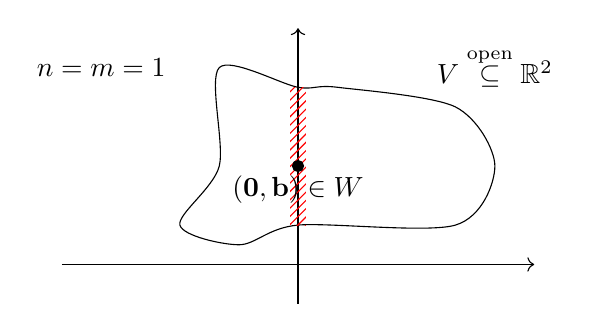
\begin{tikzpicture}
        \draw[->] (-3, 0) -- (3, 0);
        \draw[->] (0, -0.5) -- (0, 3);
        \draw plot [mark=none, smooth cycle] coordinates {(-1, 2.5) (0, 2.25) (0.5, 2.25) (2, 2) (2.5, 1.25) (2, 0.5) (0, 0.5) (-0.75, 0.25) (-1.5, 0.5) (-1, 1.25)};
        \fill[pattern=north east lines, pattern color=red] (-0.1, 2.25) rectangle (0.1, 0.5);
        \draw[fill=black] (0, 1.25) circle (2pt) node[below] {$(\mathbf 0, \mathbf b) \in W$};
        \node at (-2.5, 2.5) {$n = m = 1$};
        \node at (2.5, 2.5) {$V \overset{\text{open}}{\subseteq} \RR^2$};
      \end{tikzpicture}
    \end{figure}
    \begin{figure}[H]
      \centering
      \begin{subfigure}{0.45\textwidth}
        \centering
        \begin{tikzpicture}
          \draw[->] (-3, 0) -- (3, 0);
          \draw[->] (0, -0.5) -- (0, 3);
          \draw plot [mark=none, smooth cycle] coordinates {(-1, 2.5) (0, 2.25) (0.5, 2.25) (2, 2) (2.5, 1.25) (2, 0.5) (0, 0.5) (-0.75, 0.25) (-1.5, 0.5) (-1, 1.25)};
          \node at (2.5, 2.5) {$V$};
          \draw[fill=black] (0, 1.25) circle (2pt) node[right] {$\mathbf b$};
          \node at (0, 1.75) {$\rotatebox[origin=c]{270}{$($}$};
          \node at (0, 0.75) {$\rotatebox[origin=c]{270}{$)$}$};
        \end{tikzpicture}
      \end{subfigure}
      \begin{subfigure}{0.45\textwidth}
        \begin{tikzpicture}
          \draw[->] (-3, 0) -- (3, 0);
          \draw[->] (0, -0.5) -- (0, 3);
          \draw plot [mark=none, smooth cycle] coordinates {(-1.5, 1.75) (0, 1.25) (1.5, 0.75) (1.5, 1.75) (0, 1.25) (-1.5, 0.75)};
          \draw[fill=black] (0, 1.25) circle (2pt) node[above right] {$\mathbf b$};
        \end{tikzpicture}
      \end{subfigure}
    \end{figure}

    Choose $\mathbf y \in W$.
    \begin{align*}
      &\Leftrightarrow \quad (\mathbf 0, \mathbf y) \in V = F(U) \\
      &\Leftrightarrow \quad \exists (\mathbf x, \mathbf y) \in U \text{ s.t. } \underbrace{\mathbf F(\mathbf x, \mathbf y)}_{= (\mathbf f(\mathbf x, \mathbf y), \mathbf y)} = (\mathbf 0, \mathbf y) \\
      &\Leftrightarrow \quad \exists \mathbf x \in \RR^n \text{ s.t. } \mathbf f(\mathbf x, \mathbf y) = \mathbf 0.
    \end{align*}
    Observe that $\mathbf x$ is unique: if there exist $\mathbf x \neq \mathbf x'$ such that $\mathbf f(\mathbf x, \mathbf y) = \mathbf f(\mathbf x', \mathbf y) = \mathbf 0$ and that $(\mathbf x, \mathbf y), (\mathbf x', \mathbf y) \in U$, then $\mathbf F(\mathbf x, \mathbf y) = \mathbf F(\mathbf x', \mathbf y) = (\mathbf 0, \mathbf y)$, contradicting the bijectivity of $\mathbf F$ on $U$.
  \item[(b)] Note that so far for every $\mathbf y \in W$, we have a unique $\mathbf x = \mathbf g(\mathbf y)$ such that $(\mathbf x, \mathbf y) \in U$ and $\mathbf f(\mathbf g(\mathbf y), \mathbf y) = \mathbf 0$. In other words, $\mathbf x$ is \emph{implicitly} a function of $\mathbf y$, hence the name of the theorem.

    e.g., $y^2 + x^3 = 0 \Rightarrow x = \left(-y^2\right)^\frac{1}{3}$.

    However, $y^2 + xy + x^3 \sin x = 0$ cannot be solved explicitly as a function of $y$ but the implicit function theorem ensures that near certain $(a, b)$ such solutions exist.

    \noindent {\bf Goal:} $\mathbf g \in C^1(W)$ and $\mathbf g'(\mathbf b) = -\mathbf A_x^{-1} \mathbf A_y$, where $\mathbf g : \RR^m \to \RR^n$.

    Note that
    \[ \mathbf F : (\underbrace{\mathbf x}_{= \mathbf g(\mathbf y)}, \mathbf y) \mapsto (\underbrace{\mathbf f(\mathbf x, \mathbf y)}_{= \mathbf 0}, \mathbf y). \]
    Define
    \[ \underbrace{\Phi(\mathbf y)}_{\in C^1(W)} = (\underbrace{\mathbf g(\mathbf y)}_{\in C^1(W)}, \mathbf y) = \mathbf F^{-1}(\mathbf 0, \mathbf y). \]
    Then,
    \[ \Phi'(\mathbf y) =
    \begin{pmatrix}
      \mathbf g'(\mathbf y)_{n \times m} \\
      \mathbf I_{m \times m}
    \end{pmatrix}
    . \]
    By the inverse function theorem, we know $\mathbf F^{-1}$ is $C^1$ on $V$. Thus,
    \begin{align*}
      & \mathbf f(\underbrace{\mathbf g(\mathbf y), \mathbf y}_{= \Phi(\mathbf y)}) = \mathbf 0 \\
      \boxed{\xRightarrow[\text{rule}]{\text{chain}}} \quad & \underbrace{\mathbf f'(\Phi(\mathbf y))}_{n \times (n + m)} \Phi'(\mathbf y) = \mathbf 0 && \text{Why is $\mathbf g$ or $\Phi$ differentiable?} \\
      \Rightarrow \quad & \underbrace{\mathbf f'(\mathbf g(\mathbf y), \mathbf y)}_{n \times (n + m)}
      \begin{pmatrix}
        \mathbf g'(\mathbf y) \\
        \mathbf I
      \end{pmatrix}
      _{(n + m) \times m} = \mathbf 0.
    \end{align*}
    Set $\mathbf y = \mathbf b$; get
    \[ \underbrace{
      \begin{bmatrix}
        \mathbf A_x & \mathbf A_y
      \end{bmatrix}
    }_{= \mathbf f'(\underbrace{\mathbf g(\mathbf b)}_{= \mathbf a}, \mathbf b)}
    \begin{pmatrix}
      \mathbf g'(\mathbf b) \\
      \mathbf I
    \end{pmatrix}
    = \mathbf 0; \]
    i.e.,
    \[ \mathbf A_x \mathbf g'(\mathbf b) + \mathbf A_y = \mathbf 0 \quad \Rightarrow \quad \mathbf g'(\mathbf b) = -\mathbf A_x^{-1} \mathbf A_y \qquad \text{since $\mathbf A_x$ is known to be invertible}. \]
  \end{enumerate}
\end{proof}

\end{document}
